\documentclass[conference]{IEEEtran}
\IEEEoverridecommandlockouts
% The preceding line is only needed to identify funding in the first footnote. If that is unneeded, please comment it out.
\usepackage{cite}
\usepackage{amsmath,amssymb,amsfonts}
\usepackage{algorithmic}
\usepackage{graphicx}
\usepackage{textcomp}
\usepackage{xcolor}
\def\BibTeX{{\rm B\kern-.05em{\sc i\kern-.025em b}\kern-.08em
    T\kern-.1667em\lower.7ex\hbox{E}\kern-.125emX}}
\begin{document}

\title{Equilivest: A Robotic Vest to aid in Post-Stroke Dynamic Human Balance Rehabilitation
\thanks{Identify applicable funding agency here. If none, delete this.}
}

\author{\IEEEauthorblockN{1\textsuperscript{st} Franco Paviotti}
\IEEEauthorblockA{\textit{Bioingeniería} \\
\textit{Instituto Tecnológico de Buenos Aires}\\
Buenos Aires, Argentina \\
fpaviotti@itba.edu.ar}
\and
\IEEEauthorblockN{2\textsuperscript{nd} Esteban Buniak}
\IEEEauthorblockA{\textit{Ingeniería en Informática} \\
\textit{Instituto Tecnológico de Buenos Aires}\\
Buenos Aires, Argentina \\
ebuniak@itba.edu.ar}
\and
\IEEEauthorblockN{3\textsuperscript{rd} Rodrigo Ramele}
\IEEEauthorblockA{\textit{Ingeniería en Informática} \\
\textit{Instituto Tecnológico de Buenos Aires}\\
Buenos Aires, Argentina \\
rramele@itba.edu.ar}
\and
\IEEEauthorblockN{4\textsuperscript{th} Juan Miguel Santos}
\IEEEauthorblockA{\textit{Ingeniería en Informática} \\
\textit{UNAHUR}\\
Hurlingham, Argentina \\
jsantos@gmail.com}
\and
\IEEEauthorblockN{5\textsuperscript{th} Given Name Surname}
\IEEEauthorblockA{\textit{Ingeniería en Informática} \\
\textit{Instituto Tecnológico de Buenos Aires}\\
Buenos Aires, Argentina \\
fpaviotti@itba.edu.ar}
\and
\IEEEauthorblockN{6\textsuperscript{th} Given Name Surname}
\IEEEauthorblockA{\textit{Ingeniería en Informática} \\
\textit{Instituto Tecnológico de Buenos Aires}\\
Buenos Aires, Argentina \\
fpaviotti@itba.edu.ar}
}



\maketitle

\begin{abstract}
This document is a model and instructions for \LaTeX.
This and the IEEEtran.cls file define the components of your paper [title, text, heads, etc.]. *CRITICAL: Do Not Use Symbols, Special Characters, Footnotes, 
or Math in Paper Title or Abstract.
\end{abstract}

\begin{IEEEkeywords}
Stroke, Balance, Rehabilitation, Biofeedback, Vibrotactile
\end{IEEEkeywords}

\section{Introduction}

Brain stroke is a devastating disease, that affects world population and is the main cause of disabilities worldwide~\cite{Caplan.etal2023}.  Disabilities related to stroke can affect motor pathways, and may lead to several motor function disorders.   One important aspect of motor function is balance which is the ability to control the center of mass of the body inside the base support provided by the lower limb.  Stroke can affect dynamic balance as well,  which is manifested while walking and that affect autonomy, independence and is an important factor in activities of daily living (ADL) particularly for young patients~\cite{Afrasiabifar.etal2020,Donato.etal2016}.

% As early as possible the rehabilitation can be put into place, better the outcome that can be obtained by the treatment. 

Strong evidence suggests that neuroplasticity can be enhanced by neural rehabilitation~\cite{DeAngelis.etal2021,Albert.etal2012}.  These procedures are aimed to relearn movements that can trigger new pathway generation which reroute, or even completely replace, those pathways that were damaged by the stroke.  Neurorehabilitation procedures are performed by a group of interdisciplinary caregivers and technicians.  Recently, biofeedback techniques, aiming at providing extra information to the patient that can be used to aid in the relearning have appeared as an alternative treatment to increase neuralplasticitly. These are in the form of Wearable devices-based biofeedback rehabilitation (WDBR)~\cite{Peake.etal2018} or more advanced robotic rehabilitation gait devices~\cite{Zhao.etal2022,Peshkin.etal2005,Tong.etal2006}.  

%This published evidence emphasizes that this biofeedback can indeed enhance the results of rehabilitation procedures.

The working hypothesis is as follows:  the addition of an independent and new peripheral therapeutic signal, that can be assimilated as an extrasensory input,  could improve dynamic balance performance on stroke patients which may have yet insufficiency to deal properly with the complexities of walking.  The idea is that we have now the ability to provide meaningful balance information with hardware and software that can provide this extra signal in the form of any form of stimulation, particularly vibrotactile feedback (VF).  Although the effectiveness of biofeedback on static balance has been tackled extensively in the literature, works dealing with dynamic balancing problems have been negligible.

This work presents the development of a device which is grounded on this idea, and aims to help a post-stroke patient with a remaining dynamic balance problem, and present it as a case study.  The proposed development is implemented as a smart-vest~\cite{Brandebusemeyer.etal2021}, which we will call, equilivest, that address three possible clinical hypothesis of the underlying problem.  We aim to provide motor learning, meaning to provide a fading vibrotactile feedback signal which is as less conscious as possible~\cite{Donato.etal2016}.  The device aims to promote plasticity by providing timing vibrotactile stimulation based on kinematic and dynamics measurements.  

%The idea is to exploits these ideas from neurofeedback that we can create "external" sensors by providing some form of vibrotactile stimulation on her belly and link that stimulation to some form of measurements from IMUs (inertial sensors).

%The form of validation procedures that is required in clinical settings\cite{Papastylianou.etal2016}.

Section presents the case study.  Next section summarize the results of the interviews and surveys performed by the patient, their family and professional caregivers.  Based on the analyze of the data, the next section presents the underlying clinical hypothesis. Section A describes the vest details and architecture.  The experimental design protocol is expounded in Section B.  Preliminary results are presented on the next section, and this work concludes with discussion and conclusion.

\section{Materials and Methods}

\subsection{Single Patient Case Study}

Patient is a 31 years old female, perfectly healthy, who suffered an acute brainstem stroke after giving birth  The stroke was on posterior fossa subarachnoid due to a brain artereovenous malformation (AVM), which was likely affected by pregnancy or puerperium~\cite{Porras.etal2017}.  Patient was in coma for around 2 months, and after that unable to walk, move, talk or swallow.  After two years of intensive rehabilitation, Patient managed to recover significantly, including from dysphagia, which were very important in order to remove the feeding tube allowing her to start speech recovering.  

After 24 months since event, the patient, was discharged from hospital and only maintained a 3 times per week rehabilitation treatment, focusing on a remaining affection related with dynamic walking balance problems.  The patient achieved satisfactory index scores in static balance tests and is fully able to perform hip-balance and ankle-balance.  She has recovered muscle in her legs and can perform lower-limb exercises.  Her vision is normal.   Tests performed to verify proprioceptive system were successfully passed.

However, when the patient tries to walk on open-spaces, or with confronting lights (like walking towards sunlight), with other people moving around, or when walking concentration fades, she is unable to keep up with the pace of the gait and falls frequently.  This is consistent, under these situations.  Nowadays, the patient can walk with a Canadian cane or a non-actuated walking helper which she is hesitant to use, both.

\begin{table*}[t]
\begin{center}
\begin{tabular}[!t]{|c|c|}
\hline
Question & Avg. answer \\
\hline
Podes describir cómo y cuándo se expresa la perdida del equilibrio y su proceso? - Esta pregunta nos servirá para determinar con mayor precisión los métodos de sensado y alarma a desarrollar  & Cuando estoy cansada, distraída o muy nerviosa\\
\hline
¿Siempre se desarrolla de la misma manera? - Con esta pregunta queremos profundizar sobre la anterior con el objetivo de una mejor comprensión &  Si \\
\hline
¿Cuál? Si la respuesta fue no, deje sin contestar  & Me desequilibro\\
\hline
¿Podés evidenciar cuando estas por empezar a perder el equilibrio? - Con esta pregunta intentamos conocer un fenómeno que permita detectar el principio de caída & Si \\
\hline
Si la respuesta fue si ¿Qué sentís? & Un poco no siempre siento inestabilidad previo  \\
\hline
¿Con qué frecuencia usas el andador? - Puede seleccionar mas de una opción. Así nos ayudará a entender mejor el cuadro & Solo fuera de casa \\
\hline
¿Existe algún denominador común en las caídas? - La presencia de este sería importantísima para  un fenómeno o señal a medir y caracterizar que sería muy útil para la detección del principio de caídas. Si hay algo que siempre se repite podríamos enfocarnos en detectar eso. & Si \\
\hline\\
¿Cuál? Si la respuesta fue "No" deje la respuesta en blanco & Lo que anteriormente dije estoy cansada o distraída o nerviosa  \\
\hline
¿Cómo estás trabajando la recuperación hoy por hoy? - Con esta pregunta buscamos conocer el estado de situación y trabajo actual & Fortalecimiento de músculos   \\
\hline
¿Hay algo más que desees comentar o expresar? & No uso andador es un bastón canadiense. 
Ahora me doy cuenta antes que me voy a caer, pero queda poco para evitarlo.   \\
\hline
\end{tabular}
\caption{table}{Answers to survey questions.}
\label{tab:alpi_q_table_1}
\end{center}
\end{table*}



\begin{table*}[t]
\begin{center}
\begin{tabular}[!t]{|c|c|}
\hline
Question & Avg. answer \\
\hline
¿Cuál es la razón de la pérdida del equilibrio en la paciente? - Esta pregunta nos permite conocer la opinión de los profesionales e interiorizarnos en el caso.  & Lesión en el tronco del encéfalo\\
\hline
¿Podes describir cómo y cuándo se expresa la perdida del equilibrio y su proceso? - Con la descripción podemos comprender como y en que circunstancias se desencadena el fenómeno de la caída y conocer mejor el caso. &  La pérdida del equilibrio se expresa en el inicio y durante la marcha. cuando se detiene también. Camina con compensación visual y cuando quita la vista el suelo (ej mira para el costado aumenta la inestabilidad) Realiza una marcha sin el automatismo habitual. Le demanda mucha concentracion.  \\
\hline
¿ La paciente puede caminar sin un dispositivo de tipo ayuda marcha? De ser así, ¿Bajo que circunstancias? - Conociendo mejor la situación actual podemos tomar mejores decisiones en cuanto a como posicionar sensores y medir.  & Solo de manera  terapéutica. habitualmente la trabajamos con máxima supervisión.\\
\hline
¿Presenta una pérdida de fuerza muscular que dificulte el caminar? - Esta pregunta permite conocer el caso en mayor detalle  con propiedad para evitar adelantarnos a hipótesis de trabajo erróneas. & No \\
\hline
¿Presenta dismetría? - Nuevamente queremos adelantarnos a hipótesis erróneas a la hora de decidir el método de sensado y procesamiento de las señales. La longitud o duración de los movimientos puede usarse como un indicador para nosotros, como también asi los ritmos. & Si \\
\hline
¿Presenta temblores?  - En caso de presentar temblores estos se verán reflejados en las señales y es útil tenerlo en cuenta ya que caracterizará a nuestra señal. & No \\
\hline
¿Presenta alteraciones en la marcha en instantes previos a la caída? - En caso de existir algún impulso inicial que podamos sensar o medir de forma indirecta podemos anticiparnos a la perdida del equilibrio en las señales. & Si \\
\hline\\
¿Cuáles? Si la respuesta fue "No" deje en blanco & Fallas las reacciones de tobillo y cadera \\
\hline
¿Sufrió alteraciones en la sensibilidad profunda? - Existe un trabajo previo en la Universidad de Buenos Aires que usa un método de sensado orientado a la presión de la pisada. Esto puede orientarnos en otro sentido en el sensado y estimulación. & No  \\
\hline
Antes de perder el equilibrio, ¿Trastabilla?¿Acelera la marcha? -  Al igual que en otras preguntas buscamos obtener información extra para el  procesamiento de las señales y detección del principio de caída. Estos fenómenos pueden medirse o detectarse y evidenciarían el inicio de una posible caída. & Otro síntoma  \\
\hline
Si la respuesta fue 'Otro síntoma' ¿Cuál? - En caso contrario deje sin responder & Reacción lenta \\
\hline
¿Presenta algún tipo de marcha patológica? -la caracterización del caso permite decidir formas y métodos de sensado y procesamiento. & Si  \\
\hline
¿Cuál? Si la respuesta fue "No" deje la respuesta en blanco & Marcha Atáxica \\
\hline
¿Existe algún denominador común en las caídas? - La presencia de este sería importantisima para  un fenómeno o señal a medir y caracterizar que sería muy útil para la detección del principio de caídas. Si hay algo que siempre se repite podríamos enfocarnos en detectar eso. & Si \\
\hline
¿Cuál? Si la respuesta fue "No" deje la respuesta en blanco & El denominador es cuando deja de realizar la marcha de manera consciente. Por ejemplo, cuando camina y tiene que realizar alguna tarea que implique procesos cognitivo. Dual Task  \\
\hline
¿Se hizo un estudio de evaluación de marcha? - Esta pregunta podría aportar información suplementaria a preguntas anteriores que nos permiten conocer e interiorizarnos en el caso & No  \\
\hline
¿Se hizo evaluación de riesgo de caídas? - Esta pregunta puede aportar algo de información extra para el conocimiento del caso. & Si  \\
\hline
¿Hay alguna manera en que trabaje en la reeducación de la paciente? -  Quisiéramos conocer un poco mas la situación actual y las actividades que realiza la paciente para su recuperación. & Si a través de la reeducación del VOR,  facilitación del equilibrio estático y dinámico, entrenamiento del automatismo de la marcha con diferentes niveles de dificultad.  \\
\hline
¿Hay algo mas que desee comentar o expresar?  & Mes a mes se evidencia una mejora, todavía no alcanza para que pueda caminar sin supervisión.  \\
\hline
\end{tabular}
\caption{table}{Answers to survey questions.}
\label{tab:alpi_q_table_1}
\end{center}
\end{table*}

Based on the surveys and the information provided by caregivers there seems not to be any somatosensorial deficit~\cite{Donato.etal2016}. 
There isn't any report of somatosensorial on foot sole. 


\subsection{Underlying hypothesis}

Human balance is composed of a complex interaction of different subsystems, which includes somatosensorial information, vestibular system and visual information as input sources.  These are later processed in different networks of the Central Nervous System, and finally actuated by motor pathways at many different scales~\cite{Donato.etal2016}.

We perform a series of surveys and interviews with the patient and their caregivers.  Main results are summarized in 
Tables ~\ref{tab:patientsurvey} and \ref{tab:caregiverssurvey}.  Based on the clinical history, the results from the surveys and interviews, we postulate three different potential clinical situations that could use the external signal in the form of biofeedback and could potentially aid in rehabilitation procedures.

%Bradykinesia: due to the slow speech.
%Unusual gait
%Dysmetria (visual?) (ataxia?)

\begin{itemize}
\item Vestibular information or fusion of vestibular information
\item Bradykinesia: the processing speed required to effectively perform the processing and actuation is not enough.
\item Unusual gait: due to ataxic gait the movement is not normally regulated.
\end{itemize}


\subsection{Robotic Device Vest}
The whole vest system is made of, in a high level description, a battery shield, an esp8266 based arduino shield, an inertial measurement unit (MPU 6050) and a vibration motor to stimulate the patient. MPU 6050 uses the accelerometer and gyroscope data to get angular acceleration and measure pitch roll and yaw angles. Said angles are measured by calculation with the corresponding equations and processed with a complementary filter which relies 80\% in gyroscope data and 20\% in accelerometer data. This values will be sent in real time as packets to a UDP server and later visualized and exported by the server host for further processing. The whole system can be powered by power banks or a 18650 battery array.

\textbf{Why only vibrotactile stimulation and not auditory stimulation}

\subsection{Experimental Design}

Three experiments were designed in order to test each one of the hypothesis.  All the experiments were approved by the ITBA University ethical committee.  Participants were recruited voluntarily.

%\begin{itemize}
%\item Controlamos que la posición del IMU no supere un umbral, y si lo hace vibra el motor.
%\item Intentamos predecir una situación de caída y generar un alerta antes de que ocurra.
%\item Hacemos un pacemaker.  Es decir una estimulación sincrónica asociada a la detección de un podómetro.
%\end{itemize}

\subsubsection{Vestibular Feedback}

The underlying idea is that signals from IMU can be feed back to the patient by vibrotactile stimulation on their belly.  The hypothesis is that if there is a vestibular problem that forbids the patient to receive or evaluate the vestibular information appropriately, this external signal can be available for the patient to integrate it into the dynamic balance integration.

In order to test it, 5 healthy participants are going to be recruited to simulate falling breakpoint conditions on the IMU information.  Participants wear the vest and perform a forward walking exercise with the upper-trunk leaned forward at different angles progresively until they can no longer cope with the unbalance situation without stepping forward.

Afterward, the experiment will be repeated with the 5 participants activating the vibrotactile stimulation which will map progressively the inclination angle.  Hence it will provide an extra signal that can give a accurate information in relation to the stability of the upper-trunk in relation to the walking gait.

\subsubsection{Bradykinesia: Fall prediction due to insufficient speed of step}

All the IMU information represent a multichannel time series.  Hence, it can be used to predict a falling situation.   

In this case, 5 healthy participants perform 20 controlled falls over gym mats.  

%(3) Ver en base a la encuesta como se da la situación de caída más común que Paula relata, en base a lo que ella manifiesta.  Entonces lo que hacemos es tomamos 5 sujetos y los hacemos caer 5 veces cada uno sobre la colchoneta (o 10 o 20 x sujeto, lo que más puedas).  Con estos datos, que son series de tiempo de 6 variables, intetamos ver si con un modelo de ML podemos predecir el momento de la caída simulada de cada uno de ellos y ANTICIPARNOS .  La idea entonces es que suene el motor cuando el sistema detecta con antelación que puede venir una caída inminente.  Aca se muestra el accuracy en la detección de la caída en los datos recabados.

\subsubsection{Gait Pacemaker}

This is a gait pacemaker coupled with a podometer.  It has been showed that gait synchronization with music achieved better effect \cite{Roerdink.etal2007} and there are effect on gait trainer on patient \cite{Blicher.etal2009}.   During this experiment 5 participants walked 5 meters distance.  IMU information was obtained to derive standard diagrams of gait patterns.  They were compared against those obtained for the patient under study.  And it was determiend the exact moment when the deviation against the patient was greater and the VF was triggered upon that.

%(4) En este caso, lo que hacemos es armar un gráfico de gait y lo que hace el dispositivo es detectar un punto en el ciclo y vibrar de forma recurrente, como un marca paso, basado en un podómetro.  En este caso, tomás 5 personas las hacés caminar, determinás cómo son esas curvas y accionás el motor siempre en el mismo momento.  Lo que mostramos son los gráficos y el momento donde se dispara la estimulación.


\subsection{Participants}

Participants are recruited voluntarily and the experiment is conducted anonymously in accordance with the declaration of Helsinki published by the World Health Organization. No monetary compensation is handed out and all participants agree and sign a written informed consent approved by the ITBA University Research Commission.

%\subsection{Abbreviations and Acronyms}\label{AA}
%Define abbreviations and acronyms the first time they are used in the text, 
%even after they have been defined in the abstract. Abbreviations such as 
%IEEE, SI, MKS, CGS, ac, dc, and rms do not have to be defined. Do not use 
%abbreviations in the title or heads unless they are unavoidable.
%
%\subsection{Units}
%\begin{itemize}
%\item Use either SI (MKS) or CGS as primary units. (SI units are encouraged.) English units may be used as secondary units (in parentheses). An exception would be the use of English units as identifiers in trade, such as ``3.5-inch disk drive''.
%\item Avoid combining SI and CGS units, such as current in amperes and magnetic field in oersteds. This often leads to confusion because equations do not balance dimensionally. If you must use mixed units, clearly state the units for each quantity that you use in an equation.
%\item Do not mix complete spellings and abbreviations of units: ``Wb/m\textsuperscript{2}'' or ``webers per square meter'', not ``webers/m\textsuperscript{2}''. Spell out units when they appear in text: ``. . . a few henries'', not ``. . . a few H''.
%\item Use a zero before decimal points: ``0.25'', not ``.25''. Use ``cm\textsuperscript{3}'', not ``cc''.)
%\end{itemize}
%
%\subsection{Equations}
%Number equations consecutively. To make your 
%equations more compact, you may use the solidus (~/~), the exp function, or 
%appropriate exponents. Italicize Roman symbols for quantities and variables, 
%but not Greek symbols. Use a long dash rather than a hyphen for a minus 
%sign. Punctuate equations with commas or periods when they are part of a 
%sentence, as in:
%\begin{equation}
%a+b=\gamma\label{eq}
%\end{equation}
%
%Be sure that the 
%symbols in your equation have been defined before or immediately following 
%the equation. Use ``\eqref{eq}'', not ``Eq.~\eqref{eq}'' or ``equation \eqref{eq}'', except at 
%the beginning of a sentence: ``Equation \eqref{eq} is . . .''
%
%\subsection{\LaTeX-Specific Advice}
%
%Please use ``soft'' (e.g., \verb|\eqref{Eq}|) cross references instead
%of ``hard'' references (e.g., \verb|(1)|). That will make it possible
%to combine sections, add equations, or change the order of figures or
%citations without having to go through the file line by line.
%
%Please don't use the \verb|{eqnarray}| equation environment. Use
%\verb|{align}| or \verb|{IEEEeqnarray}| instead. The \verb|{eqnarray}|
%environment leaves unsightly spaces around relation symbols.
%
%Please note that the \verb|{subequations}| environment in {\LaTeX}
%will increment the main equation counter even when there are no
%equation numbers displayed. If you forget that, you might write an
%article in which the equation numbers skip from (17) to (20), causing
%the copy editors to wonder if you've discovered a new method of
%counting.
%
%{\BibTeX} does not work by magic. It doesn't get the bibliographic
%data from thin air but from .bib files. If you use {\BibTeX} to produce a
%bibliography you must send the .bib files. 
%
%{\LaTeX} can't read your mind. If you assign the same label to a
%subsubsection and a table, you might find that Table I has been cross
%referenced as Table IV-B3. 
%
%{\LaTeX} does not have precognitive abilities. If you put a
%\verb|\label| command before the command that updates the counter it's
%supposed to be using, the label will pick up the last counter to be
%cross referenced instead. In particular, a \verb|\label| command
%should not go before the caption of a figure or a table.
%
%Do not use \verb|\nonumber| inside the \verb|{array}| environment. It
%will not stop equation numbers inside \verb|{array}| (there won't be
%any anyway) and it might stop a wanted equation number in the
%surrounding equation.
%
%\subsection{Some Common Mistakes}\label{SCM}
%\begin{itemize}
%\item The word ``data'' is plural, not singular.
%\item The subscript for the permeability of vacuum $\mu_{0}$, and other common scientific constants, is zero with subscript formatting, not a lowercase letter ``o''.
%\item In American English, commas, semicolons, periods, question and exclamation marks are located within quotation marks only when a complete thought or name is cited, such as a title or full quotation. When quotation marks are used, instead of a bold or italic typeface, to highlight a word or phrase, punctuation should appear outside of the quotation marks. A parenthetical phrase or statement at the end of a sentence is punctuated outside of the closing parenthesis (like this). (A parenthetical sentence is punctuated within the parentheses.)
%\item A graph within a graph is an ``inset'', not an ``insert''. The word alternatively is preferred to the word ``alternately'' (unless you really mean something that alternates).
%\item Do not use the word ``essentially'' to mean ``approximately'' or ``effectively''.
%\item In your paper title, if the words ``that uses'' can accurately replace the word ``using'', capitalize the ``u''; if not, keep using lower-cased.
%\item Be aware of the different meanings of the homophones ``affect'' and ``effect'', ``complement'' and ``compliment'', ``discreet'' and ``discrete'', ``principal'' and ``principle''.
%\item Do not confuse ``imply'' and ``infer''.
%\item The prefix ``non'' is not a word; it should be joined to the word it modifies, usually without a hyphen.
%\item There is no period after the ``et'' in the Latin abbreviation ``et al.''.
%\item The abbreviation ``i.e.'' means ``that is'', and the abbreviation ``e.g.'' means ``for example''.
%\end{itemize}
%An excellent style manual for science writers is \cite{b7}.
%
%\subsection{Authors and Affiliations}
%\textbf{The class file is designed for, but not limited to, six authors.} A 
%minimum of one author is required for all conference articles. Author names 
%should be listed starting from left to right and then moving down to the 
%next line. This is the author sequence that will be used in future citations 
%and by indexing services. Names should not be listed in columns nor group by 
%affiliation. Please keep your affiliations as succinct as possible (for 
%example, do not differentiate among departments of the same organization).
%
%\subsection{Identify the Headings}
%Headings, or heads, are organizational devices that guide the reader through 
%your paper. There are two types: component heads and text heads.
%
%Component heads identify the different components of your paper and are not 
%topically subordinate to each other. Examples include Acknowledgments and 
%References and, for these, the correct style to use is ``Heading 5''. Use 
%``figure caption'' for your Figure captions, and ``table head'' for your 
%table title. Run-in heads, such as ``Abstract'', will require you to apply a 
%style (in this case, italic) in addition to the style provided by the drop 
%down menu to differentiate the head from the text.
%
%Text heads organize the topics on a relational, hierarchical basis. For 
%example, the paper title is the primary text head because all subsequent 
%material relates and elaborates on this one topic. If there are two or more 
%sub-topics, the next level head (uppercase Roman numerals) should be used 
%and, conversely, if there are not at least two sub-topics, then no subheads 
%should be introduced.
%
%\subsection{Figures and Tables}
%\paragraph{Positioning Figures and Tables} Place figures and tables at the top and 
%bottom of columns. Avoid placing them in the middle of columns. Large 
%figures and tables may span across both columns. Figure captions should be 
%below the figures; table heads should appear above the tables. Insert 
%figures and tables after they are cited in the text. Use the abbreviation 
%``Fig.~\ref{fig}'', even at the beginning of a sentence.
%
%\begin{table}[htbp]
%\caption{Table Type Styles}
%\begin{center}
%\begin{tabular}{|c|c|c|c|}
%\hline
%\textbf{Table}&\multicolumn{3}{|c|}{\textbf{Table Column Head}} \\
%\cline{2-4} 
%\textbf{Head} & \textbf{\textit{Table column subhead}}& \textbf{\textit{Subhead}}& \textbf{\textit{Subhead}} \\
%\hline
%copy& More table copy$^{\mathrm{a}}$& &  \\
%\hline
%\multicolumn{4}{l}{$^{\mathrm{a}}$Sample of a Table footnote.}
%\end{tabular}
%\label{tab1}
%\end{center}
%\end{table}
%
%\begin{figure}[htbp]
%\centerline{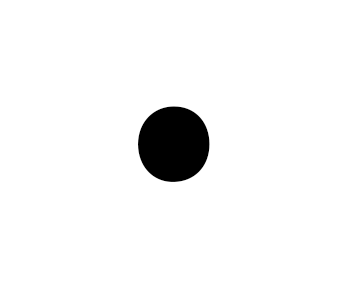
\includegraphics{fig1.png}}
%\caption{Example of a figure caption.}
%\label{fig}
%\end{figure}
%
%Figure Labels: Use 8 point Times New Roman for Figure labels. Use words 
%rather than symbols or abbreviations when writing Figure axis labels to 
%avoid confusing the reader. As an example, write the quantity 
%``Magnetization'', or ``Magnetization, M'', not just ``M''. If including 
%units in the label, present them within parentheses. Do not label axes only 
%with units. In the example, write ``Magnetization (A/m)'' or ``Magnetization 
%\{A[m(1)]\}'', not just ``A/m''. Do not label axes with a ratio of 
%quantities and units. For example, write ``Temperature (K)'', not 
%``Temperature/K''.

\section*{Results}

(1) Se muestran entonces esos dos gráficos promediados de cada uno de los 5 sujetos (10 series, 5 sin el motor, 5 con el motor).


(2) Se muestra los gráficos de las series de tiempo offline de los datos analizados y como el sistema online de predicción acierta justamente en anticipar la caída.  (Esto es probablmente desde software lo más complejo).

(3) Este caso probablemente sea el que requiera más experimentación sobre Paula en sí misma.  La idea acá es tener los gráficos promediados de GAIT, que son todos cíclicos, de dos de las variables cualquiera del IMU que formen un ciclo, y ver que hay un patrón común que se da más o menos para las personas healthy.  En base a eso, luego la idea es probar si con Paula ese patrón CAMBIA.  A partir de que vemos si cambia hay que ver donde cambia y en ese punto meter el pacemaker.

\section*{Discussion}



\section*{Conclusion}

This device used as a testbed can be extended easily to provide biofeedback which also aim to increase the effectiveness of rehabilitation procedures~\cite{Bowman2021}.


\section*{Acknowledgment}

%The preferred spelling of the word ``acknowledgment'' in America is without 
%an ``e'' after the ``g''. Avoid the stilted expression ``one of us (R. B. 
%G.) thanks $\ldots$''. Instead, try ``R. B. G. thanks$\ldots$''. Put sponsor 
%acknowledgments in the unnumbered footnote on the first page.

%Please number citations consecutively within brackets \cite{b1}. The 
%sentence punctuation follows the bracket \cite{b2}. Refer simply to the reference 
%number, as in \cite{b3}---do not use ``Ref. \cite{b3}'' or ``reference \cite{b3}'' except at 
%the beginning of a sentence: ``Reference \cite{b3} was the first $\ldots$''
%
%Number footnotes separately in superscripts. Place the actual footnote at 
%the bottom of the column in which it was cited. Do not put footnotes in the 
%abstract or reference list. Use letters for table footnotes.
%
%Unless there are six authors or more give all authors' names; do not use 
%``et al.''. Papers that have not been published, even if they have been 
%submitted for publication, should be cited as ``unpublished'' \cite{b4}. Papers 
%that have been accepted for publication should be cited as ``in press'' \cite{b5}. 
%Capitalize only the first word in a paper title, except for proper nouns and 
%element symbols.
%
%For papers published in translation journals, please give the English 
%citation first, followed by the original foreign-language citation \cite{b6}.

\bibliographystyle{IEEEtran}
\bibliography{iros}


%
%\vspace{12pt}
%\color{red}
%IEEE conference templates contain guidance text for composing and formatting conference papers. Please ensure that all template text is removed from your conference paper prior to submission to the conference. Failure to remove the template text from your paper may result in your paper not being published.

\end{document}
